\reportheading{5. VAV zoning and duct layout (Task 3)}
{\centering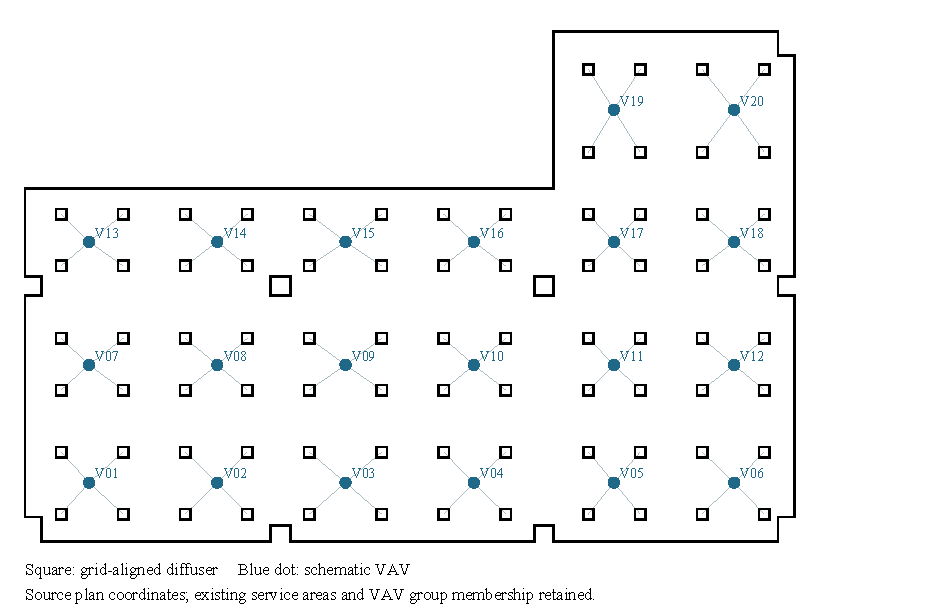
\includegraphics[width=.82\linewidth]{figures/layout.pdf}\par}
\reportfigure{}{Figure 3. Grid-aligned diffuser arrangement and twenty four-outlet VAV groups.}
Each panel occupies a full ceiling tile within its assigned service cell. Each VAV serves four outlets. The source-coordinate layout in Figure 3 defines the directional lengths in Appendix B.


\subhead{5.1 Supply route to the office wing}
The supply trunk leaves the air-handling unit through A-01, A-02 and A-03. At the trunk split, D-22 and D-23 carry 1549.78 L/s for both wing boxes. After the take-off, D-24 carries the remaining 766.49 L/s to D-44, the final rigid connection to VAV-20. Four flexible runs serve SD-75, SD-76, SD-79 and SD-80. Appendix C gives their combined minimum flow as 306.6 L/s.

At the VAV-19 take-off, the required rigid section reduces from 600 × 400 mm on D-23 to 450 × 300 mm on D-24. At that point the branch carries only the four outlets served by VAV-20. The VAV-20 plan connections span 2.918–3.083 m. Adding the 0.50 m routing allowance to the longest gives 3.583 m, within the adopted 4 m cap and the 5 m project limit. Final routing must maintain clearance and avoid fire-resisting barriers [1].

{\centering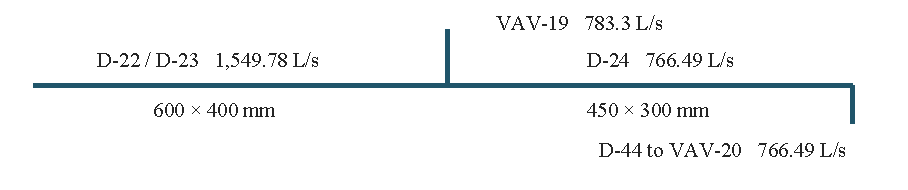
\includegraphics[width=\linewidth]{figures/wing-flow.pdf}\par}
\reportfigure{}{Figure 4. Peak airflow at the wing take-off. The remaining branch serves VAV-20.}
At the take-off, 783.3 L/s leaves the shared run for VAV-19. The flow continuing to VAV-20 divides again at the box: SD-75 and SD-76 each receive 189.46 L/s, SD-79 receives 202.19 L/s and SD-80 receives 185.40 L/s. Their sum accounts for the branch duty to the precision shown on the drawing.
